

\documentclass[14pt]{report}
\usepackage[a4paper]{geometry}
\usepackage[myheadings]{fullpage}
\usepackage{fancyhdr}
\usepackage{lastpage}
\usepackage{graphicx, wrapfig, subcaption, setspace, booktabs}
\usepackage[T1]{fontenc}
\usepackage[font=small, labelfont=bf]{caption}
\usepackage{fourier}
\usepackage[protrusion=true, expansion=true]{microtype}
\usepackage[english]{babel}
\usepackage{sectsty}
\usepackage{url, lipsum}
\usepackage{tgbonum}
\usepackage{hyperref}
\usepackage{xcolor}
\usepackage{minted}
\usepackage[utf8]{inputenc}
\newcommand{\HRule}[1]{\rule{\linewidth}{#1}}
\onehalfspacing
\setcounter{tocdepth}{5}
\setcounter{secnumdepth}{5}


%-------------------------------------------------------------------------------
% HEADER & FOOTER
%-------------------------------------------------------------------------------
\pagestyle{fancy}
\fancyhf{}
\setlength\headheight{15pt}
\fancyhead[L]{Simone Berni }
\fancyhead[R]{Fondamenti di Computer Graphics}
%-------------------------------------------------------------------------------
% TITLE PAGE
%-------------------------------------------------------------------------------

\begin{document}

{\fontfamily{cmr}\selectfont
\title{ \normalsize \textsc{}
		\\ [2.0cm]
		\HRule{2pt} \\ [0.5cm]
	    \textbf{\uppercase{Corso di Fondamenti di Computer Graphics}}\\
		\HRule{0.5pt} \\
		\LARGE \textbf{\uppercase{Report Laboratori}
		\HRule{2pt} \\ [0.5cm]
		\normalsize \today \vspace*{5\baselineskip}}
		}

\date{}

\author{
        \textbf{Simone Berni 893034} \\
        Laurea Magistrale in Informatica\\
        Alma Mater Studiorum
 }

\maketitle
\newpage

%-------------------------------------------------------------------------------
% Section title formatting
%-------------------------------------------------------------------------------

%-------------------------------------------------------------------------------
% BODY
%-------------------------------------------------------------------------------
\section*{Introduzione}
Tutte le seguenti esercitazioni sono state svolte utilizzando come sistema operativo Arch Linux e come ide CLion della IntelliJ. Se ci dovessero essere problemi di incompatibilità con i sistemi Windows, mi scuso, ma purtroppo tutte le mie macchine girano su sistemi Unix.
% PANDA scorretto in ita. Scrivi "in tutte le mie macchine girano sistemi Unix"
\newpage

%PANDA ti prego togli lo 0 prima, non si può vedere, anche nell'indice
\section*{Esercitazione 1}
\texttt{Consegne}
\begin{enumerate}
    \item Compilare e far girare il programma. Provare i controlli da keyboard. Il left mouse button aggiunge
un punto. I comandi 'f' e 'l' rimuovono il primo e l’ultimo punto dalla lista di punti, rispettivamente.
Oltre ai 64 punti, i primi punti sono rimossi.
    \item Osservare come il programma usa le OpenGL GLUT callback per catturare gli eventi click del
mouse e determinare le posizioni (x, y) relative.
    \item Provare a cambiare lo stile di punti e linee.
    \item Disegnare la curva di Bézier a partire dai punti di controllo inseriti, utilizzando l’evaluator di
OpenGL ( glMap1f(), glMapGrid1f(), glEvalMesh1()). Ricordarsi di abilitare il disegno di curve con glEnable(GL\_MAP1\_VERTEX\_3)
    \item Sostituire alle routine di OpenGL il disegno della curva mediante algoritmo di de Casteljau.
    \item Integrare nel programma in alternativa uno dei seguenti punti:
(a) disegno di una curva di Bézier mediante algoritmo ottimizzato basato sulla suddivisione adattiva.
(b) disegno interattivo di una curva di Bézier composta da tratti cubici, dove ogni tratto viene
raccordato con il successivo con continuitá C 0 , C 1 , o G 1 a seconda della scelta utente da
keyboard.
    \item Permettere la modifica della posizione dei punti di controllo tramite trascinamento con il mouse
\end{enumerate}
 \texttt{Svolgimento}
 \begin{enumerate}
     \item Nulla da dover descrivere
     \item Nulla da dover descrivere
     \item È possibile cambiare la dimensione della linea modificando il valore all'interno della funzione \textit{glLineWidth}. La dimensione dei punti invece è modificabile attraverso la chiamata a \textit{glPointSize}
     \item Il codice dell'implementazione è verificabile nel sorgente sotto la funzione \textit{drawBezierGL}, ma descrivendolo brevemente, è sufficiente utilizzare le funzioni di liberia \textit{glBegin} per iniziare a disegnare i punti, i quali verranno calcolati attraverso la funzione \textit{glEvalCoord1f}. 
     \item L'algoritmo di Casteljau è stato implementato nel seguente modo ed è verificabile nel sorgente sotto la funzione \textit{castelAlgo}:\\ 
     Per ogni valore del parametro \textit{t}, si effettuano una serie di LERP, e se i punti di controllo sono N, allora per ogni valore si effettuano $$\sum_{i=0}^{n} lerp$$, dove con lerp si intende l'interpolazione lineare, calcolata come Lerp(t,A,B)=(1-t)A+tB.\\
     A questo punto, è possibile disegnare la curva utilizzando una chiamata a \textit{glVertex3f}.
    \item E' stato scelto di integrare il punto A, utilizzare cioè la suddivisione adattiva per implementare la curva di Bezier. Anche in questo caso il sorgente è consultabile, sotto le funzioni \textit{drawBezierAdaptive} e \textit{adaptiveSubdivision}.\\
    In questo caso non viene dato il parametro \textit{t} nel quale deve essere valutata la curva, come nelle fasi precedenti, bensì un valore di tolleranza.
    La prima parte consiste nel calcolare la distanza di ogni punto dalla corda tra il primo e l'ultimo punto e, se la distanza di ogni punto intermedio è minore della tolleranza, allora la curva può essere approssimata con una linea retta.\\
    Di questa parte si occupano le prime righe del codice, in particolare \textit{pointLineDistance} che
    permette il calcolo della distanza tra ogni punto e la corda e, in caso positivo, cioè con distanza minore dalla tolleranza, si disegnano i punti con le primitive di OpenGL.\\
    In caso negativo invece, la curva viene splittata in due, aggiungendo i punti calcolati con la LERP, e il processo è iterato per le due sottocurve ricorsivamente, finchè non è possibile disegnare l'intera curva.
    \item L'implementazione è stata effettuata attraverso due callback, chiamate \textit{passive} e \textit{motion}.
    La seconda viene invocata quando avviene un drag di un punto, e si occupa di modificare le coordinate dell'elemento e di invocare la funzione di display. In realtà è invocata
    ogni volta che il mouse si muove sullo schermo, ma effettua veramente del lavoro solo quando l'utente ha cliccato un punto, grazie alla variabile \textit{isMoving}.\\
    \textit{Passive} invece ha un compito diverso, quello di identificare che l'utente stia passando sopra ad un punto di controllo o no. In caso positivo, colora il punto di controllo in cui si trova di colore rosso, distinguendolo dagli altri. Per fare ciò si calcola la distanza della posizione dal mouse da tutti i punti sullo schermo e, in caso sia minore di una certa tolleranza, marca il punto e invoca la funzione di display, che si occuperà del colore.\\
           {\centering
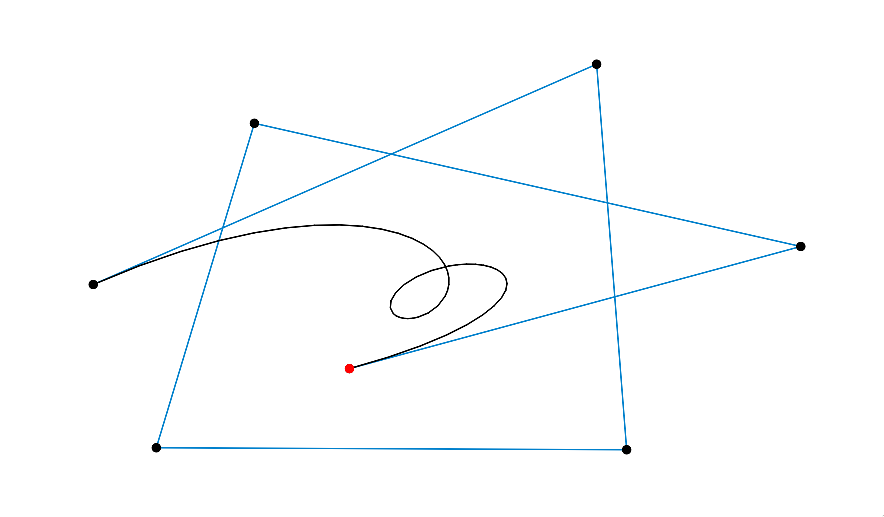
\includegraphics[width=0.6\textwidth]{bezier.png}} 
 \end{enumerate}

\section*{Esercitazione 2}
\texttt{Consegna}\\
Si richiede di realizzare una demo di animazione digitale 2D interattiva simile al materiale fornito.\\
Punti fondamentali del progetto:
\begin{itemize}
    \item l’impegno artistico e l’impatto visivo della scena
    \item la presenza e qualitá delle animazioni basate su simulazioni fisiche (es. uso leggi di cinematica/
dinamica)
    \item la presenza di elementi di gameplay con condizioni di vittoria/sconfitta per il giocatore
    \item l’utilizzo dei particellari nella scena
\end{itemize}
\texttt{Svolgimento}\\
Creazione di Arkanoid.\\
La demo creata consiste in un livello di Arkanoid, il cui scopo è colpire tutti i mattoncini con una palla. L'implementazione, in quanto doveva essere un breve gioco, consiste di un solo livello. \\
Analizzando ora tutti i punti fondamentali richiesti nel progetto:
\begin{itemize}
    \item Le animazioni che sono state utilizzate all'interno del gioco sono tre: il movimento della pallina quando rimbalza su una superficie, il movimento del giocatore, e la scomparsa di un blocco quando esso viene colpito.\\
    \begin{itemize}
        \item Per rendere la pallina controllabile, quando viene colpita dal giocatore, il nuovo angolo che avrà la pallina varia in base alla posizione di dove ha colpito il giocatore. È stata utilizzata la formula della interpolazione lineare per trovare il nuovo angolo. Per capire come è stata utilizzata la LERP per risolvere questo problema, è sufficiente consultare la funzione \textit{playerBallAngle}
        \item Il giocatore non ha accelerazione, ma si muove con velocità costante, altrimenti sarebbe incontrollabile e sarebbe impossibile colpire la pallina nel punto voluto
        \item I blocchi una volta colpiti, non scompaiono veramente, ma il loro colore diventa uguale a quello dello sfondo e non vengono più considerati gli impatti con quel blocco
    \end{itemize}
    \item Sinceramente, non trovo le particelle molto belle visivamente, ma data la richiesta, sono state emesse all'impatto della pallina con il giocatore.
    \item Ci sono due possibilità per il giocatore: vincere o perdere. In ogni caso, lo schermo finale sarà il medesimo, ma la prima possibilità la si ottiene colpendo tutti i blocchi, la seconda facendo cadere la pallina. Per conoscere il proprio punteggio è stato inserito lo score dei blocchi distrutti attualmente.\\
           {\centering
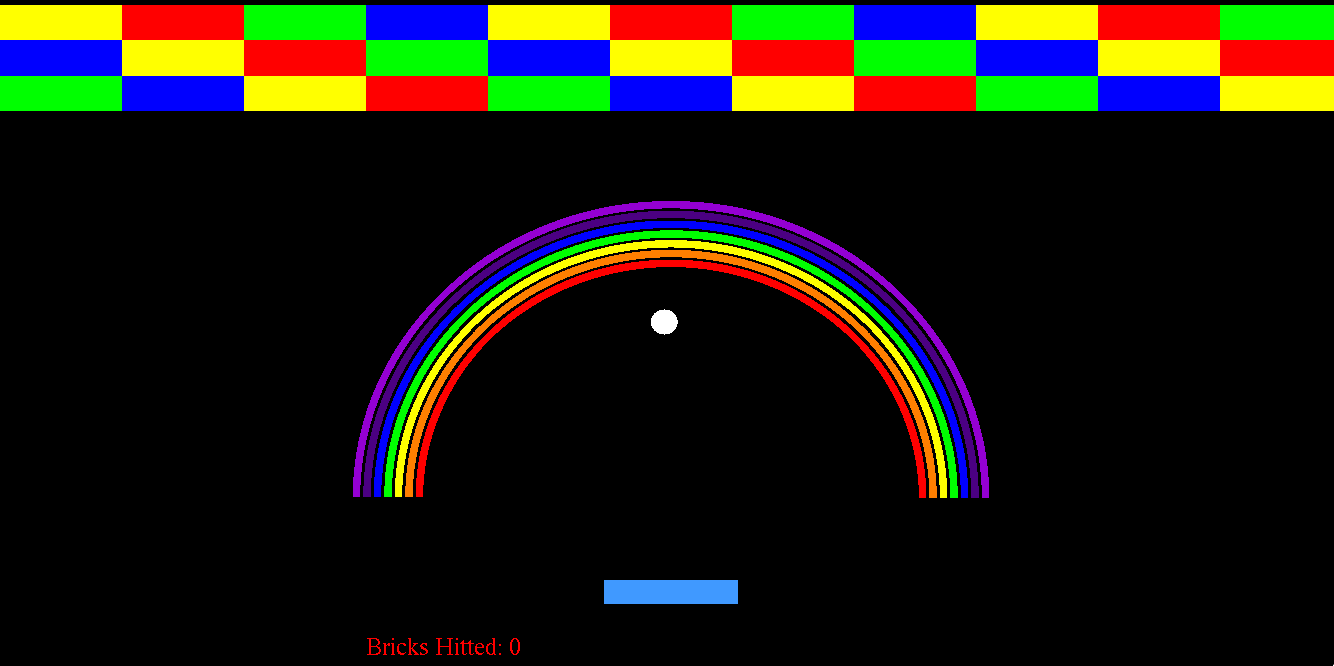
\includegraphics[width=0.6\textwidth]{arkanoin.png}} 
\end{itemize}

\section*{Esercitazione 3}
\texttt{Consegna:}
\begin{enumerate}
    \item Caricamento e visualizzazione modelli mesh poligonali
    \begin{enumerate}
        \item Caricamento e visualizzazione di più di un oggetto mesh con la possibilità di passare la selezione dall'uno all'altro tramite special key
        \item Verifica della gestione della visualizzazione dei modelli poligonali tramite VAO/VBO
        \item Calcolo e memorizzazione delle normali ai vertici per i modelli mesh poligonali. Visualizzazione con normali ai vertici in modalità smooth
        \item Permettere il cambio di materiale dell'oggetto da pop-up menù
    \end{enumerate}
    \item Navigazione interattiva in scena
    \begin{enumerate}
        
        \item Pan orizzontale camera
        \item Pan verticale camera
        \item Zoom camera
        \item Culling
        \item Smooth/Flat shading
        \item Materials
        \item Camera Motion
    \end{enumerate}
    \item Trasformazione degli oggetti in scena
    \begin{enumerate}
        \item Traslazione, Rotazione, Scalatura WCS/OCS
    \end{enumerate}
    
\end{enumerate}
\texttt{Svolgimento:}\\
Parto dal presupposto che ho dovuto commentare la generazione della sfera(luce) dal codice, perchè per una qualche ragione non ancora ben identificata, con quella matrice sul mio computer con OS Arch non visualizzo più nessun oggetto. 
Su Ubuntu invece, mi funzionava anche con quella riga di codice, sinceramente non ho capito la motivazione.\\ Inoltre, per poter testare, è necessario cambiare
il path di \textbf{MeshDir}, in quanto la mia architettura richiedeva un path assoluto e non relativo.
\begin{enumerate}
    \item Caricamento e visualizzazione modelli mesh poligonali
    \begin{enumerate}
        \item Ogni oggetto è, al momento della inizializzazione, caricato utilizzando la funzione \textit{createMesh}, che inserisce l'oggetto all'interno di un array. Il controllo di quale elemento mostrare in ogni momento, è gestito grazie alla variabile \textbf{selectedObject} e dalla funzione \textit{drawOne}
        \item Nulla da dover descrivere
        \item  La richiesta è stata implementata aumentando le funzioni \textit{generate\_and\_load\_buffers} e \textit{loadObjFile}
        \item E' stata implementata la funzione \textit{material\_menu\_function} che, dato il valore dell'opzione cliccato,
        modifica il tipo di materiale dell'oggetto in questo momento selezionato
    \end{enumerate}
    \item Navigazione interattiva in scena
    \begin{enumerate}
    
        \item Le funzioni che si occupano dello spostamento a destra e sinistra sono rispettivamente \textit{moveCameraRight} e \textit{moveCameraLeft}.
        Per risolvere la richiesta, è necessario modificare la posizione della camera e del target, di uno stesso valore. In particolare, il vettore che si occupa di quantificare lo spostamento è un vettore a 4 dimensioni con valori 1,0,-1,0. Per spostarsi a sinistra il vettore è stato sommato a quello che identifica la posizione del target e della camera, per lo spostamento a destra sono stati sottratti.
        \item Le funzioni che si occupano dello spostamento in alto e in baso sono rispettivamente \textit{moveCameraUp} e \textit{moveCameraDown}. Per risolvere la richiesta, è necessario modificare la posizione della camera e del target, di uno stesso valore. In particolare, il vettore che si occupa di quantificare lo spostamento è un vettore a 4 dimensioni con valori 1,0,-1,0. Per spostarsi in alto il vettore è stato sommato a quello che identifica la posizione del target e della camera, per lo spostamento in basso sono stati sottratti.
        \item Le funzioni che si occupano dello zoom in avanti e indietro sono rispettivamente \textit{moveCameraForward} e \textit{moveCameraBack}. L'idea delle due funzioni è la stessa, cambia solo la costante che indica il movimento, da 1 a -1. L'implementazione segue la regola della retta parametrica passante per un punto. Si prende il vettore che va dal punto target alla posizione attuale. Il valore delle componenti sarà positivo se ci si vuole avvicinare al target, negativo altrimenti. A questo punto si aggiorna la posizione sommando quella attuale con il vettore, moltiplicato per una costante che ne indica la quantità di spostamento. 
        \item E' sufficiente invocare rispettivamente \textit{glEnable} e \textit{glDisable} del valore \textbf{GL\_CULL\_FACE} per abilitare o disabilitare il culling
        \item E' sufficiente invocare \textit{gkShadeModel} con il valore \textbf{GL\_FLAT} \textbf{GL\_SMOOTH} per abilitare rispettivamente il flat shading o lo smooth shading
        \item La funzione è stata implementata per la consegna 1.4
        \item  L'idea è avere n punti di controllo, tali che il primo e l'ultimo abbiano le stesse coordinate, e muovere la telecamera sulla curva di bezier da loro creata, utilizzando l'algoritmo creato nella esercitazione 1. Il codice è consultabile nella funzione \textit{cameraMotion}. Per creare l'animazione, è stata utilizzata la funzione di libreria \textit{glutIdleFunction}. Dato che i punti sono fissi, se si sposta l'oggetto dalla posizione 0,0,0, non ci si muoverà attorno all'oggetto, ma attorno alla sua posizione iniziale.\\
           {\centering
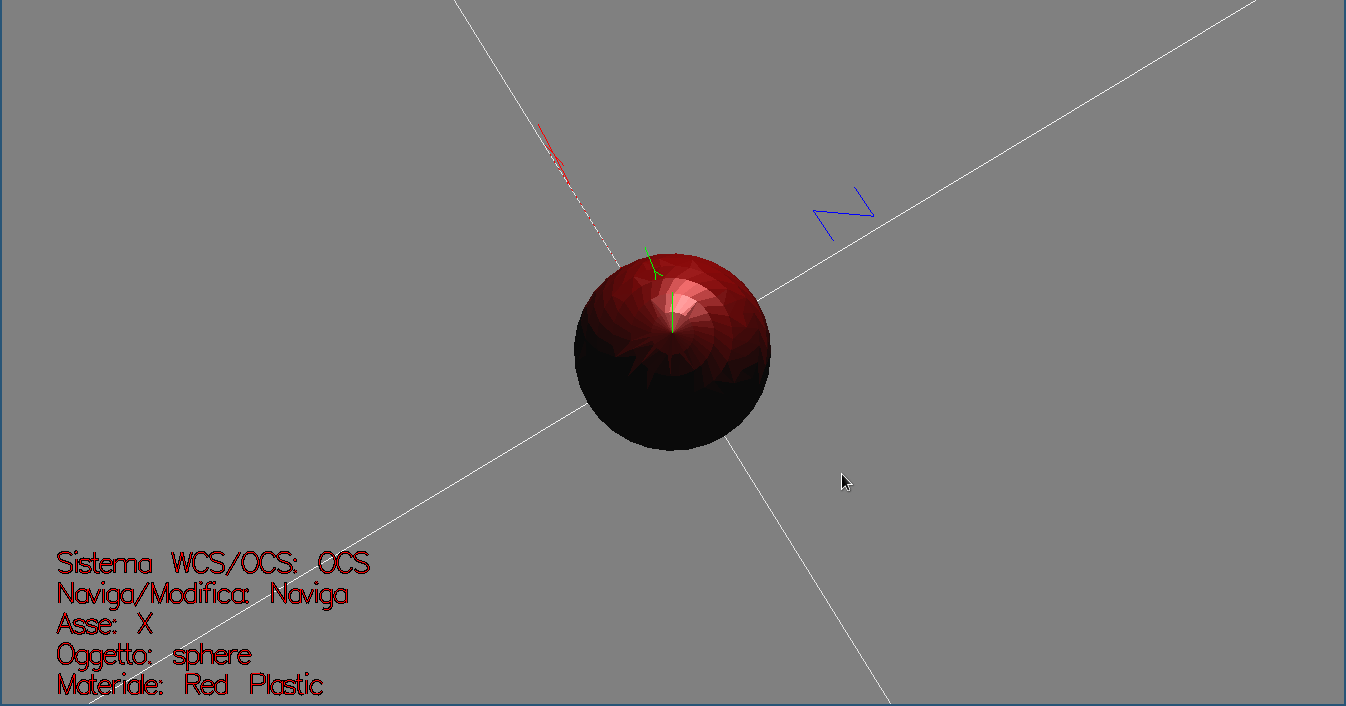
\includegraphics[width=0.6\textwidth]{moveAround.png}} 
    \end{enumerate}
    \item Trasformazione degli oggetti in scena
    \begin{enumerate}
        \item Per ottenere la posizione attuale dell'oggetto, si moltiplica l'identità per la matrice dell'oggetto, per effettuare la traslazione si può utilizzare la funzione \textit{GlTransaltef}, per la rotazione la funzione \textit{glRotatef} e infine per la scalatura \textit{glScalef}. Per questa ultima funzione non ho capito se si dovesse scalare un asse alla volta, oppure no. Personalmente ho preferito implementare la scalatura dell'oggetto in sè, in quanto la consideravo più utile, ma se fosse stato necessario scalare un asse alla volta, è sufficiente modificare i parametri di \textit{glScalef} controllando l'asse di lavoro. La differenza tra WCS e OCS consiste semplicemente nell'ordine delle operazioni svolte, come è possibile verificare nella funzione \textit{modifyModelMatrix}\\
           {\centering
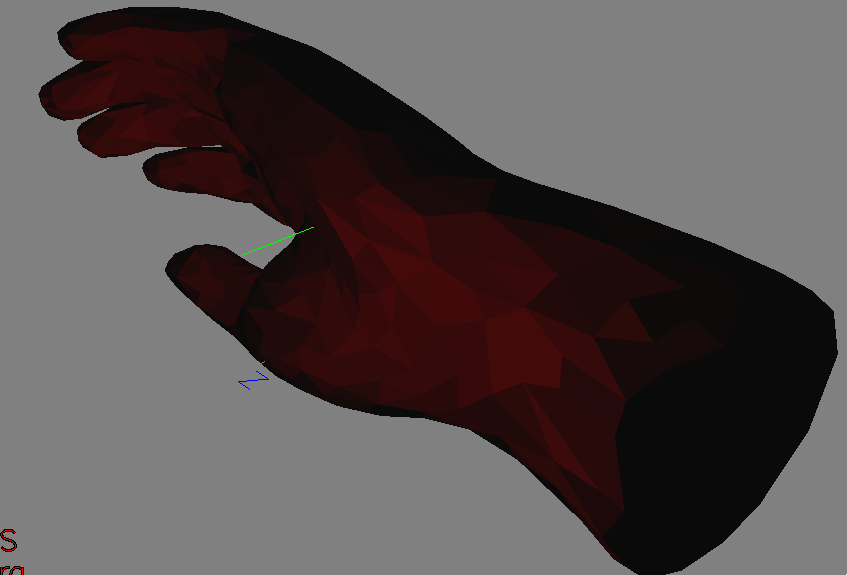
\includegraphics[width=0.6\textwidth]{manoTrasl.png}} 
    \end{enumerate}
    
\end{enumerate}


\section*{Esercitazione 6} 
\texttt{Consegna:}
\begin{enumerate}
    \item \textbf{Lighting}: permettere lo spostamento interattivo della luce posizionale/direzionale in scena
    \item \textbf{Shading}: realizzare la modalità shading Phong realizzando gli shaders \texttt{v\_phong.glsl} e \texttt{f\_phong.glsl} 
    \item \textbf{Texture mapping 2D} del toro con immagine letta da file utilizzando gli shaders \texttt{v\_texture.glsl} e \texttt{f\_texture.glsl}.
    \item \textbf{Texture mapping 2D + Shading} Realizzare gli shaders \texttt{v\_texture\_phong.glsl} e \texttt{f\_texture\_phong.glsl} per combinare l'effetto shading Phong con la texture image sulla mesh toro
    \item \textbf{Procedural mapping} basato su un procedimento algoritmico a piacere sul toro
    \item \textbf{Wave Motion} creare l'animazione dell'oggetto \textit{GridPlane} modificando la posizione dei vertici in un vertex shader \texttt{v\_wave.glsl}. Utilizzando la variabile elapsed time \textit{t}, passata da applicazione al vertex shader, per riprodurre il moto ondoso ottenuto con la sola modifica della coordinata y.
    \item \textbf{Toon Shading}: realizzare gli shaders \texttt{v\_toon.glsl} e \texttt{f\_toon.glsl} per la resa non fotorealistica nota comunemente come Toon Shading
    
\end{enumerate}
\texttt{Svolgimento:}
Nuovamente è stato trovato un problema di compatibilità, in particolare la versione utilizzata negli shader. Per farli funzionare nella mia macchina, ho deciso di settarli a 320 es, ma questo ha provocato un ulteriore problema, la mancanza di precisione. Quest'ultimo punto è stato risolto inserendo la linea di codice \textit{\#precision mediump float}. La scelta del medium è per avere ulteriori problemi di compatibilità, in caso dovessi cambiare architettura hardware.\\ Nuovamente, sono stati inseriti dei path assoluti, precisamente \textbf{MeshDir}, \textbf{TextureDir} e \textbf{ShaderDir}, che devono essere modificati per testare il programma.
\begin{enumerate}
    \item \textbf{Lighting}: Selezionando l'oggetto luce, e selezionando una \textit{OperationMode} diversa dalla \textbf{Navigazione}, si arriverà ad invocare la funzione \textit{modifyModelMatrix}. Il suo contenuto è lo stesso della esercitazione3, a differenza che in questo caso non abbiamo una matrice di float, ma un mat4, ma il ragionamento dietro è lo stesso. All'interno della funzione vi è stata aggiunta la parte per la gestione anche della luce vera e propria, modificandone la posizione grazie all'attributo \texttt{light.position}.\\ Ma ciò non è sufficiente a notare, durante l'esecuzione, un cambiamento. Questo perché nella funzione \textit{display} non venivano modificati, di volta in volta, il contenuto di \textbf{light\_uniforms[SHADER]}, ma erano stati assegnati solo durante l'inizializzazione degli shaders. Aggiungendo quelle righe a tutti gli shader, è stato possibile completare la consegna.
    \item \textbf{Shading}: l'algoritmo di Phong è stato implementato negli shader\texttt{v\_phong.glsl} e \texttt{f\_phong.glsl}, e per capire come programmare uno shader sono stati utilizzati gli shaders di Blinn e Gouraud come esempi.
    \\
           {\centering
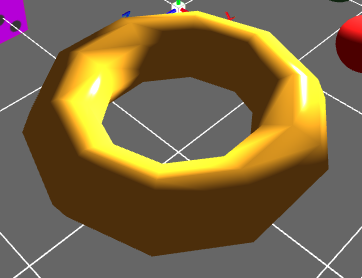
\includegraphics[width=0.6\textwidth]{toroPhong.png}} 
    \item \textbf{Texture mapping 2D}: dopo aver modificato la funzione \textit{init\_torus} con gli appositi parametri, mi sono reso conto che ciò non era sufficiente, in quanto la texture non veniva applicata correttamente. Per questo è stato aggiunto alla funzione \textit{computeTorusVertex} l'inizializzazione delle coordinate Texture.
    \\
           {\centering
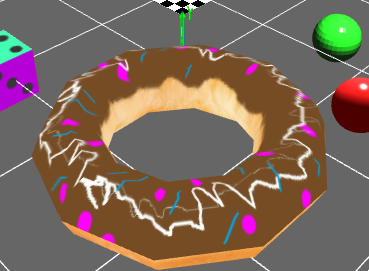
\includegraphics[width=0.6\textwidth]{toroTexture.png}} 
    \item \textbf{Texture mapping 2D + Shading}: nuovamente sono stati presi come base due shaders per creare quello richiesto, \textbf{Texture\_Only}, dato già nella esercitazione, e Phong, creato per un punto precedente.  \\
           {\centering
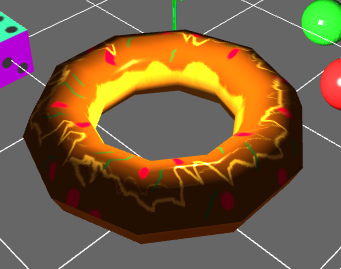
\includegraphics[width=0.6\textwidth]{toroTexturePhong.png}} 
    \item \textbf{Procedural mapping} Utilizzando la funzione \textit{generate\_texture}, che era già presente perla generazione della texture scacchiera su un piano,
    sono state create due funzioni, \textit{generateShadesOfGray} e \textit{generateRainbowMap}. La prima mi è servita per capire come lavorare sul toro, e come la texture veniva mappata sul toro. La seconda, esteticamente magari più piacevole, mi ha permesso di capire come modificare i colori nella zona selezionata.\\
          {\centering
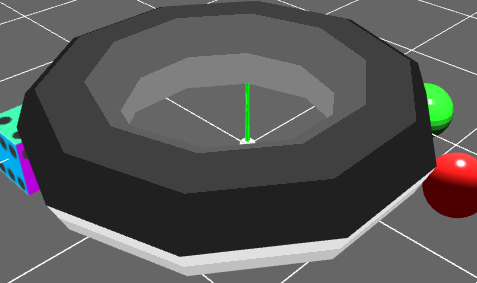
\includegraphics[width=0.6\textwidth]{toroGrey.png}}\\
{\centering
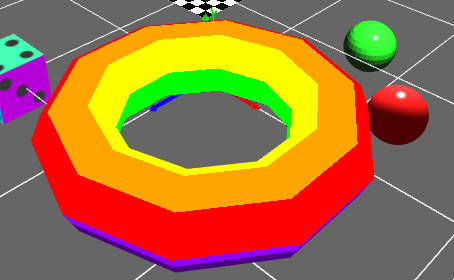
\includegraphics[width=0.6\textwidth]{toroArcobaleno.png}}
    \item \textbf{Wave Motion}: La costruzione prevede varie parti: la prima è l'inizializzazione della wave, effettuata nella funzione \textit{init\_wave}. Successivamente c'è la parte di configurazione dello shader, simile agli altri, con solo la differenza che gli viene passato anche il parametro \textit{t}, richiesto dall'esercizio e ottenuto attraverso \textit{glutGet(GLUT\_ELAPSED\_TIME)}. Per poter attivare il movimento è stata aggiunta una nuova opzione nel menù, \textbf{Move waves}, che attiverà \textit{glutIdleFunc} della mia callback, \textit{moveWaves}. Questa funzione non fa altro che richiamare costantemente lo shader sull'oggetto, con il nuovo valore di \textbf{waveTime}.\\ Lo shader è abbastanza lineare, come il vertex shader \texttt{v\_passthrough.glsl} ottiene la posizione e, applicando la formula inserita nella richiesta dell'esercitazione, calcola la nuova posizione. Sono state aggiunte anche le righe di codice necessarie al passaggio di una texture, in quanto mi sembrava troppo brutto lasciarlo bianco.\\
        {\centering
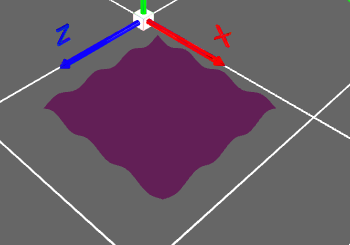
\includegraphics[width=0.6\textwidth]{wave.png}}
    \item \textbf{Toon Shading} L' idea per creare il toon shading è abbastanza semplice: si considerano intervalli fissi di luce, nel mio caso sono 4 intervalli limitati dai valori 30, 60 e 80 e ogni punto, a seconda della intensità della luce che lo colpisce, viene reso più luminoso moltiplicando il colore base per un valore costante a seconda dell'intervallo in cui cade. Il resto del codice di  \texttt{v\_toon.glsl} e \texttt{f\_toon.glsl}  è lo stesso degli altri shaders. \\
    {\centering
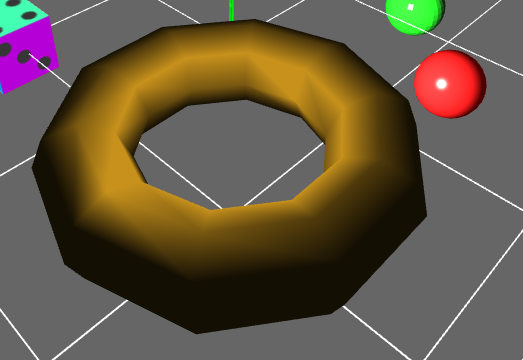
\includegraphics[width=0.6\textwidth]{toroToon.png}}

\end{enumerate}
% PANDA ciao poci ciao

}
\end{document}
